%-------------------------------------------------------------------------------
%	PAQUETES Y OTRAS CONFIGURACIONES
%-------------------------------------------------------------------------------

%-------------------------------------------------------------------------------
%	PAQUETES Y OTRAS CONFIGURACIONES
%-------------------------------------------------------------------------------
\documentclass{tufte-handout}
%\documentclass[paper=letter, fontsize=11pt]{scrartcl} % Tamaño de papel y letra para el documento
\usepackage{geometry}
\geometry{left=1.2cm, right=6.2cm, top=2.5cm, bottom=2.5cm}
\usepackage{color}
\usepackage[utf8]{inputenc} % Los caracteres acentuados se pueden escribir normalmente en el código
\usepackage[T1]{fontenc} % Configuración de fuente de salida
\usepackage{cmbright}
\usepackage[sfdefault]{noto}
\usepackage[T1]{fontenc}
\normalfont
\usepackage{graphicx} % Paquetes para incluir imágenes
\usepackage{multicol}
\usepackage{circuitikz}
\usepackage{tikz}
\usetikzlibrary{arrows}

\usepackage{sectsty} % Paquete para configuración de secciones
\allsectionsfont{\centering \normalfont \scshape} % Los títulos de las secciones son centrados, con la misma fuente y pequeñas mayúsculas

\usepackage{todonotes}
\usepackage{microtype}
\renewcommand{\figurename}{Figura}

\usepackage{listings}
\renewcommand{\lstlistingname}{Código}
\lstdefinestyle{mystyle}{
    basicstyle=\footnotesize,
    breakatwhitespace=false,
    breaklines=true,
    captionpos=b,
    keepspaces=true,
    numbers=left,
    numbersep=5pt,
    showspaces=false,
    showstringspaces=false,
    showtabs=false,
    tabsize=2
}
\lstset{style=mystyle}

% \usepackage{fancyhdr} % Paquete para personalizar pies y cabeceras de página
% \pagestyle{fancyplain} % Todas las páginas con las mismas cabeceras y pies de página
% \fancyhead{} % Sin cabecera
% \fancyfoot[L]{} % Vacío en la izquierda del pie de página
% \fancyfoot[C]{} % Vacío en el centro del pie de página
% \fancyfoot[R]{\thepage} % Número de página en el pie de pagina
% \renewcommand{\headrulewidth}{0pt} % Sin lineas en la cabecera
% \renewcommand{\footrulewidth}{0pt} % Sin lineas en el pie de página
% \setlength{\headheight}{13.6pt} % Altura de cabecera
%
% \numberwithin{equation}{section} % Numera ecuaciones en cada sección
% \numberwithin{figure}{section} % Numera figuras en cada sección
% \numberwithin{table}{section} % Numera tablas en cada sección
%
% \setlength\parindent{0pt} % Quita la indentación de los párrafos

\newcommand{\horrule}[1]{\rule{\linewidth}{#1}} % Comando personalizado para hacer linea horizontal


%-------------------------------------------------------------------------------
%	TITULO
%-------------------------------------------------------------------------------

\title{Práctica 3 - Control de motores CD\\Interfaces y periféricos para robots}
\author{Roberto Cadena Vega} % Nombre del profesor
\date{}

%-------------------------------------------------------------------------------
%	EMPIEZA EL DOCUMENTO
%-------------------------------------------------------------------------------

\begin{document}
\maketitle % Imprime el título

%-------------------------------------------------------------------------------
%	OBJETIVOS
%-------------------------------------------------------------------------------

\section{Objetivos}

	Controlar la velocidad de un motor de corriente directa de acuerdo a especificaciones enviadas por el puerto serial.

%-------------------------------------------------------------------------------
%	CONOCIMIENTOS PREVIOS
%-------------------------------------------------------------------------------

\section{Conocimientos Previos}

%-------------------------------------------------------------------------------

	\subsection{PWM}

		\begin{marginfigure}
			\begin{center}
				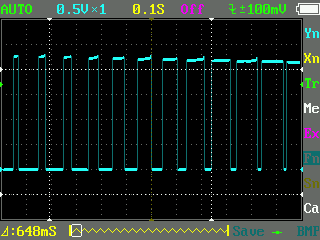
\includegraphics[width=\textwidth]{images/PWM_fade.png}
				\caption{PWM variante con el tiempo}
				\label{fig:PWM_fade}
			\end{center}
		\end{marginfigure}

		Empezaremos esta práctica analizando el concepto de una señal digital que nos permite controlar una variable que parece analógica en cualquier otro caso, el voltaje de salida del $\mu C$.

		\begin{marginfigure}
			\begin{center}
				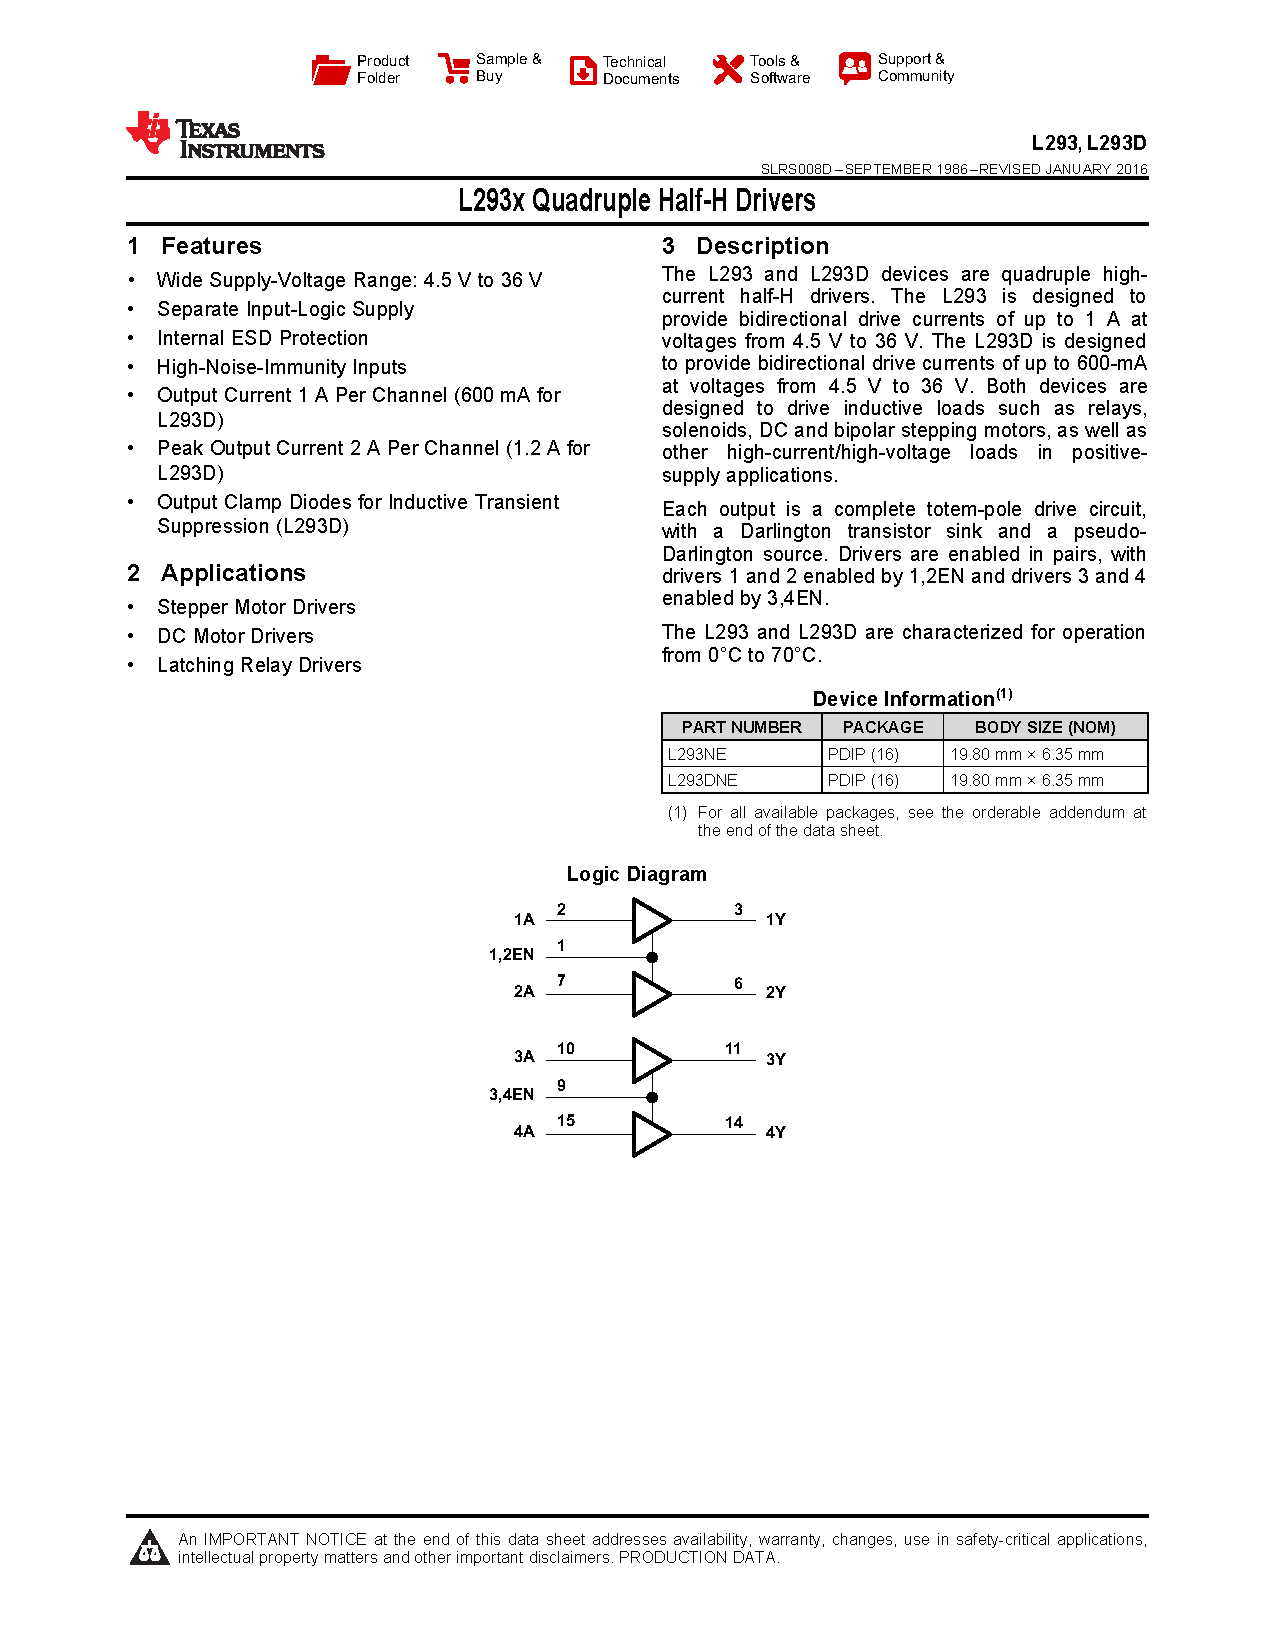
\includegraphics[width=\textwidth]{images/por_data.pdf}
				\caption{Datasheet del circuito integrado ULN2003A}
				\label{fig:data}
			\end{center}
		\end{marginfigure}

		Lo primero que haremos será modificar el código de ejemplo Fading que hemos utilizado en practicas anteriores, ya que sabemos que este genera una señal PWM para modificar la luminosidad del LED conectado a su salida:

		\lstinputlisting[language=C]{codigos/dc_motor_fade.ino}

		Si conectamos nuestro osciloscopio a la salida del Arduino, podremos ver una señal como la de la figura \ref{fig:PWM_fade}, de tal manera que la luminosidad del LED corresponde al porcentaje del tiempo que la señal permanece en un estado de $1$ lógico.

		Si ahora, estas pensando que tienes que conectar tu motor al Arduino y hacer que gire, espera... lo único que cnoseguiras será quemar tu Arduino y probablemente el puerto USB de la computadora. Tenemos que asegurarnos que la corriente que demanda el motor no pase por el Arduino directamente, para esto podemos utilizar un circuito como el ULN2003A, que es un conjunto de arreglos Darlington, diseñado para dirigir corrientes de hasta $0.5A$, o bien circuitos como el L293D o el L298N que estan diseñados explicitamente para controlar motores de corriente directa.

		\begin{marginfigure}
			\begin{center}
				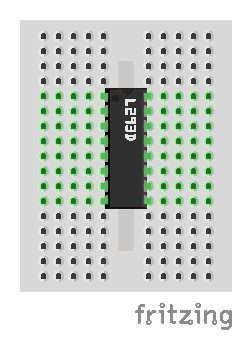
\includegraphics[width=\textwidth]{images/L293D.pdf}
				\caption{ULN2003A}
				\label{fig:CI}
			\end{center}
		\end{marginfigure}

		En esta práctica se dará como ejemplo un circuito con el ULN2003A, sin embargo tu deberás utilizar el circuito que hayas adquirido; para esto es de primera importancia que tengas a la mano el datasheet del circuito que hayas conseguido; el datasheet es un documento que describe la correcta utilización del un circuito electrónico, por lo general estos tienen caratulas como la de la figura \ref{fig:data}, el cual corresponde al ULN2003A.

		En la figura \ref{fig:data} podemos ver una representación esquemática del circuito interno del CI, ten en cuenta que cuando lo coloquemos en la protoboard, el CI se verá como en la figura \ref{fig:CI}, con una muesca en la parte superior, que corresponde a la muesca en la parte superior del diagrama esquemático del datasheet.

		Si ahora seguimos las especificaciones de conexion encontradas en el datasheet, podemos hacer nuestro circuito para controlar el motor por medio del Arduino. Nota que en la figura \ref{fig:motor_arduino}, existen dos cables que no tienen conexion, estos se tienen que conectar a una fuente de alimentación, de tal manera que esta sea la que alimente al motor y no la tajeta de desarrollo Arduino. Nota tambien que la figura tiene marcada una conexion de tierra desde el Arduino a la conexion de tierra del protoboard, esta conexion es necesaria siempre que se tengan multiples fuentes de alimentación, en este caso el Arduino y la fuente de alimentación del laboratorio.

		\begin{figure}
			\begin{center}
				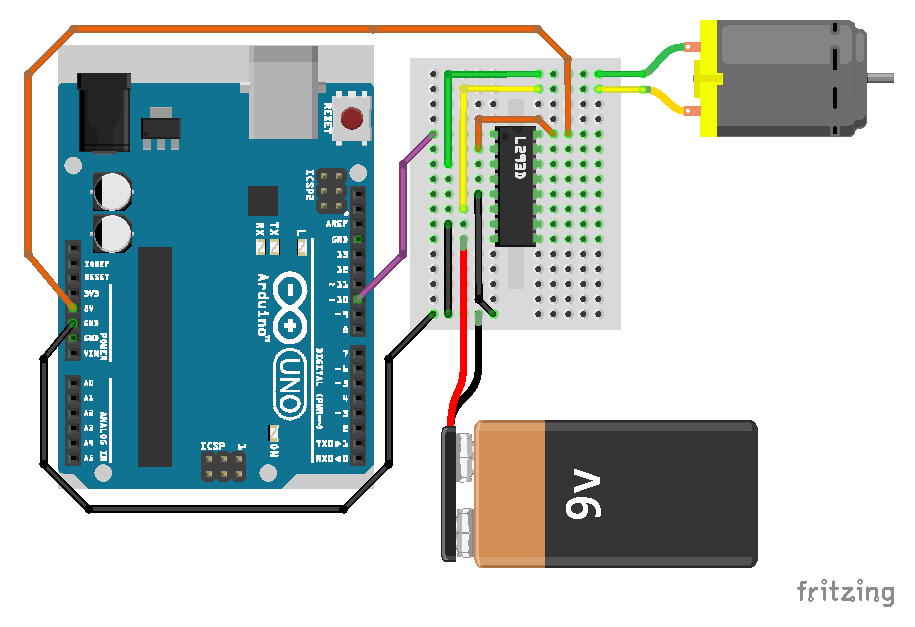
\includegraphics[width=0.8\textwidth]{images/Arduino-L293D-CD.pdf}
				\caption{Conexion Arduino - ULN2003A - Motor CD}
				\label{fig:motor_arduino}
			\end{center}
		\end{figure}

		Una vez conectado nuestro circuito podemos medir con el osciloscopio la misma señal que en la figura \ref{fig:PWM_fade} si lo conectamos a la entrada del ULN2003A, pero si lo conectamos a la salida (el punto acoplado al motor CD), veremos una señal diferente, una como la de la figura \ref{fig:PWM_fade_z}.

		\begin{marginfigure}
			\begin{center}
				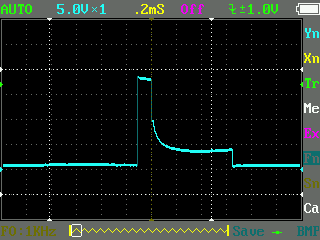
\includegraphics[width=\textwidth]{images/PWM_fade_z.png}
				\caption{Señal de alimentación cuadrada acoplada a motor CD}
				\label{fig:PWM_fade_z}
			\end{center}
		\end{marginfigure}

		En lugar de tener una señal cuadrada, podemos ver como se desestabiliza la señal hasta llegar a un valor mínimo, dependiendo de la construcción de tu motor de CD, pudieras ver un efecto similar o igual al de la figura \ref{fig:PWM_fade_z}, de cualquier manera, este efecto tiene que ver con la inductancia y reluctancia del motor, convirtiendo la señal eléctrica en una señal magnética y de regreso al sistema, otra de las razones por las que no es una buena idea conectar un motor directamente a un CI delicado como un $\mu C$.

		Para este punto queremos controlar la velocidad del motor por medio de instrucciones en la computadora, por lo que pensamos acerca de las variables involucradas en esta señal; la frecuencia de la señal de control y el porcentaje de duty cycle, empezaremos modificando la frecuencia de la señal.

		Desafortunadamente no hay una manera sencilla de modificar la frecuencia de la señal de control utilizando el código anterior, por lo que utilizaremos el siguiente:
		\newpage

		\lstinputlisting[language=C]{codigos/dc_motor_vel.ino}

		En las lineas 1-6, tenemos variables que configuran nuestra señal de control, \texttt{freq = 1000} nos da la frecuencia de $1kHz$, con lo que se calcula el periodo de la señal, el duty cycle es $30\%$ y con esto se calcula el tiempo de encendido y el tiempo de apagado; estos tiempos se utilizan en las lineas 16 y 18 para poner un retraso con estos tiempos.

		Si se pone a trabajar este código en el Arduino, veremos trabajar al motor con una cierta velocidad y oiremos un ruido muy especifico, exactamente un tono de $1kHz$, podemos modificar este código para replicar diferentes tonos, de acuerdo a la frecuencia que pongamos, o lo que es incluso mejor, si ponemos una frecuencia mayor a $20kHz$ dejaremos de escuchar este tono, la audición humana trabaja entre $20Hz$ y $20kHz$.

		Podemos hacer algo mas, con el siguiente codigo podemos modificar la frecuencia de la señal mandando datos por medio del monitor serial:

		\lstinputlisting[language=C]{codigos/dc_motor_vel_ser.ino}

		En este código se agrega una función que va a cambiar las variables de configuración de la señal de control, se manda a llamar esta función cada que hay datos nuevos mandados desde la computadora.

		%\newpage

%-------------------------------------------------------------------------------
%	EQUIPO
%-------------------------------------------------------------------------------

\section{Equipo}

	El siguiente equipo será proporcionado por el laboratorio, siempre y cuando lleguen en los primeros 15 minutos de la práctica, y hagan el vale conteniendo el siguiente equipo (exceptuando las pinzas).

	\begin{itemize}
		\item Fuente de alimentación
		\item Osciloscopio
		\item Cables BNC - Caimán
		\item Cables de alimentación
		\item Multímetro
		\item Pinzas
	\end{itemize}

%-------------------------------------------------------------------------------
%	MATERIALES
%-------------------------------------------------------------------------------

\section{Materiales}

	\begin{itemize}
		\item Protoboard
		\item Cables
		\item Motor CD
		\item LED
		\item ULN2003A, L293D, L298N, etc.
	\end{itemize}

%-------------------------------------------------------------------------------
%	DESARROLLO
%-------------------------------------------------------------------------------

\section{Desarrollo}

	Diseña los circuitos requeridos, el código necesario para que estos funciones y responde las preguntas de la hoja de anotaciones.

%-------------------------------------------------------------------------------
%	CONCLUSIONES
%-------------------------------------------------------------------------------

\section{Conclusiones}
	El alumno deberá describir sus conclusiones al final de su reporte de práctica.

%-------------------------------------------------------------------------------
%	HOJA DE ANOTACIONES
%-------------------------------------------------------------------------------

\clearpage
\section{Hoja de Anotaciones}

	\begin{enumerate}
		\item Diseña el circuito necesario para conectar tu motor al Arduino, utilizando el CI que conseguiste. \\ \vspace{7cm}
		\item Escribe el código necesario para que el motor conectado al Arduino cambie de velocidad, cuando se le envie el duty cycle por medio del monitor serial. \\
		\item Si necesito que el motor gire en el sentido contrario, ¿Que cambio tengo que hacer en el circuito que diseñaste? \\ \vspace{7cm}
		\item Escribe el código necesario para que el motor conectado al Arduino empiece a girar con la velocidad requerida en la instrucción \texttt{M3 S1000}, en donde \texttt{1000} se refiere a $1000rpm$; suponga que el motor trabaja en un rango de velocidades de $0rpm$ a $5000rpm$. El motor debe parar cuando se envia la instrucción \texttt{M5} o \texttt{M3 S0}. Cuando cada instrucción sea ejecutada, el Arduino debe mandar el texto \texttt{ok} por el puerto serial a la computadora.\\
	\end{enumerate}

	\begin{multicols}{2}
		Integrantes del equipo: \\[0.4cm]
		\horrule{0.5pt} \\[0.4cm] % Linea horizontal delgada
		\horrule{0.5pt} % Linea horizontal delgada

		Revisó: \\[1.25cm]
		\horrule{0.5pt} \\% Linea horizontal delgada
	\end{multicols}

%-------------------------------------------------------------------------------
%	FIN DEL DOCUMENTO
%-------------------------------------------------------------------------------

\end{document}
